%%%%%%%%%%%%%%%%%%%%%%%%%%%%%%%%%%%%%%%%%
% Journal Article
% LaTeX Template
% Version 1.3 (9/9/13)
%
% This template has been downloaded from:
% http://www.LaTeXTemplates.com
%
% Original author:
% Frits Wenneker (http://www.howtotex.com)
%
% License:
% CC BY-NC-SA 3.0 (http://creativecommons.org/licenses/by-nc-sa/3.0/)
%
%%%%%%%%%%%%%%%%%%%%%%%%%%%%%%%%%%%%%%%%%

%----------------------------------------------------------------------------------------
% PACKAGES AND OTHER DOCUMENT CONFIGURATIONS
%----------------------------------------------------------------------------------------

\documentclass[oneside, 11pt, a4paper]{article}
\usepackage{polski}
\usepackage[utf8]{inputenc} 
\usepackage{cite}

\usepackage{graphicx}

\usepackage{lipsum} % Package to generate dummy text throughout this template

\usepackage[sc]{mathpazo} % Use the Palatino font
\usepackage[T1]{fontenc} % Use 8-bit encoding that has 256 glyphs
\linespread{1.05} % Line spacing - Palatino needs more space between lines
\usepackage{microtype} % Slightly tweak font spacing for aesthetics

%\usepackage[hmarginratio=1:1,top=32mm,columnsep=20pt]{geometry} % Document margins
\usepackage[top=3cm, bottom=3cm, left=2.5cm, right=2.5cm, columnsep=8mm]{geometry}

\usepackage{multicol} % Used for the two-column layout of the document
\usepackage[hang, small,labelfont=bf,up,textfont=it,up]{caption} % Custom captions under/above floats in tables or figures
\usepackage{booktabs} % Horizontal rules in tables
\usepackage{float} % Required for tables and figures in the multi-column environment - they need to be placed in specific locations with the [H] (e.g. \begin{table}[H])
\usepackage{hyperref} % For hyperlinks in the PDF

%\usepackage{lettrine} % The lettrine is the first enlarged letter at the beginning of the text


\usepackage{paralist} % Used for the compactitem environment which makes bullet points with less space between them

\usepackage{abstract} % Allows abstract customization
\renewcommand{\abstractnamefont}{\normalfont\bfseries} % Set the "Abstract" text to bold
\renewcommand{\abstracttextfont}{\normalfont\itshape} % Set the abstract itself to small italic text

\renewenvironment{abstract}
               {\list{}{}%
                \item[\textbf{Streszczenie.}]\relax}
               {\endlist}



\usepackage{titlesec} % Allows customization of titles
\usepackage[labelsep=period,font=small,format=plain,labelfont=bf,textfont=up]{caption}

% \DeclareCaptionFormat{myformat}{\fontsize{10}{11}\selectfont#1#2#3}
% \captionsetup{format=myformat}

\DeclareUnicodeCharacter{00A0}{ } % solution for "Unicode char \u8:  not set up for use with LaTeX."

%\renewcommand\thesection{\Roman{section}} % Roman numerals for the sections
%\renewcommand\thesubsection{\Roman{subsection}} % Roman numerals for subsections
\titleformat{\section}[runin]{\bfseries\centering}{\thesection.}{3pt}{} % Change the look of the section titles
%\titleformat{\subsection}[]{}{}{}{}[]
\titleformat{\subsection}[runin]{\bfseries}{\thesubsection.}{3pt}{} % Change the look of the section titles
\titlespacing*{\section}{0pt}{6pt}{3pt}[0pt]
\titlespacing*{\subsection}{0pt}{3pt}{3pt}[0pt]

\usepackage{fancyhdr} % Headers and footers
\pagestyle{fancy} % All pages have headers and footers
\fancyhead{} % Blank out the default header
\fancyfoot{} % Blank out the default footer
\renewcommand{\headrulewidth}{0pt}

%\fancyhead{} % Custom header text
\fancyfoot[RO,LE]{\begin{center}\thepage\end{center}} % Custom footer text

\renewcommand{\abstractname}{Streszczenie.}    % clear the title
\renewcommand{\absnamepos}{empty} % originally center
\setlength{\parindent}{0.4cm}
%----------------------------------------------------------------------------------------
% TITLE SECTION
%----------------------------------------------------------------------------------------

\title{\vspace{15mm}\fontsize{14pt}{10pt}\selectfont\textbf{Problematyka rozproszonych systemów - przypadek \emph{Apache Cassandra}}} % Article title

\author{
{\fontsize{12pt}{1.2em}\selectfont Marek Lewandowski} \\
{\fontsize{11pt}{1.2em}\selectfont Wydział Elektroniki i Technik Informacyjnych, Politechnika Warszawska} \\
{\fontsize{11pt}{1.2em}\selectfont \href{mailto:marek.m.lewandowski@gmail.com}{marek.m.lewandowski@gmail.com}} 
\date{}
}


%----------------------------------------------------------------------------------------

\begin{document}

\maketitle % Insert title

\thispagestyle{fancy} % All pages have headers and footers

%----------------------------------------------------------------------------------------
% ABSTRACT
%----------------------------------------------------------------------------------------



%----------------------------------------------------------------------------------------
% ARTICLE CONTENTS
%----------------------------------------------------------------------------------------

\begin{multicols}{2} % Two-column layout throughout the main article text

%\begin{abstract}
\section*{Streszczenie.}

\textit{
Artykuł omawia nierelacyjne bazy danych i twierdzenia z nimi związane takie jak \emph{CAP, BASE}. W szczególności omawia cechy szczególne i budowę bazy \emph{Apache Cassandra}. \emph{Apache Cassandra} jest kanoniczną nierelacyjną bazą danych, której zrozumienie znacząco ułatwia zrozumienie większości pozostałych nierelacyjnych baz danych.
}

\section{Motywacja.}
Nierelacyjne bazy danych powstały, w celu rozwiązania nowego rodzaju problemów, którym nie były w stanie sprostać tradycyjne bazy danych. Problemy to bardzo duża, szybko przyrastająca ilość danych oraz potrzeba obsługi równie dużego obciążenia systemu.

Ilość danych, wyrażana może być, aż peta bajtach ($1PB=1000 TB$), co może sprawiać problemy jeśli chcielibyśmy obsłużyć taką ilość danych jednym komputerem. W związku z tym poruszamy się po dziedzinie klastrów serwerów, a nie pojedynczych maszyn. Pojedyncza maszyna to również pojedynczy punkt awarii. Takie i inne problemy adresowane są przez nierelacyjne bazy danych.

Często podczas omawiania nierelacyjnych baz danych przytacza się przypadek firmy \emph{Amazon}. \emph{Amazon} oświadczył, że wzrost czasu odpowiedzi w ich serwisie o 0.1 sekundy powoduje spadek sprzedaży o 1\%. Wysoka wydajność i niski czas dostępu są możliwe dzięki nierelacyjnym bazom danych oraz innym pobocznym technikom. Warto zatem pamiętać o biznesowej wartości tych rozwiązań, wiedzieć jak działają i jakim prawom podlegają.

\section{Spójność, a dostępność.}

\section{Twierdzenie CAP.}

\subsection{Zastosowanie dzisiaj.}

\section{Parametry nierelacyjnych baz danych.}

\subsection{Reguła spójności.}

\section{Apache Cassandra.}

\subsection{Liniowa skalowalność.}

\subsection{Natywny model danych.}

\subsection{Model CQL.}

\subsection{Przypadki użycia.}

\section{Motywacja.}

Zacznijmy od przedstawienia kilku powodów, dlaczego warto zdecydować się na model aktorów.
Jednym z głównych powodów, dla których tworzenie współbieżnych programów jest trudne, jest \emph{stan}, a dokładnie \emph{zmienny współdzielony stan}. Weźmy za przykład konto bankowe, w którym stanem jest aktualne saldo na rachunku. Aby operacje takie jak wpłaty, wypłaty, przelewy i inne wykonywały się poprawnie, muszą mieć dostęp do poprawnego stanu salda, a zmiany salda z tych operacji nie mogą być nadpisane przez inne operacje. Sprowadza się to do ogólnie znanej synchronizacji.

Istnieje wiele różnych technik synchronizacji. Do podstawowych należą prymitywy synchronizacyjne, takie jak:
\begin{compactitem}
\item semafory,
\item muteksy,
\item monitory.
\end{compactitem}
Każdy z nich pozwala na synchronizację, która uchroni stan, ale poprawna synchronizacja nie należy do najprostszych zadań, zwłaszcza w bardzo współbieżnych programach. Trzeba wiedzieć, w jakiej kolejności zajmować blokady, w jakiej kolejności je zwalniać; można ich zająć za dużo lub za mało, oraz trzeba wiedzieć, co tak naprawdę w danej sytuacji powinno być chronione. Łatwo w takich przypadkach popełnić błąd, który może doprowadzić do zakleszczeń, zagłodzeń lub walki o zasoby. 

Należy zauważyć, że jeśli stan nie ulega żadnych zmianom, to nie ma potrzeby synchronizacji, a zatem znikają wszystkie problemy dotyczące synchronizacji. Używanie tak niskopoziomowych mechanizmów jak wątki, blokady, semafory, jest problematyczne dla programisty, ze względu na synchronizację. Potrzeba zatem czegoś więcej, potrzeba lepszej abstrakcji, która pozwoli uniknąć niskopoziomowych problemów.

\subsection{Dostępność.}

Większość systemów powinna mieć wysoką dostępność w ciągu dnia, tygodnia, roku. W przeciwnym wypadku tracimy klientów, a co za tym idzie -pieniądze. 

Systemy mają różną rangę dostępności liczoną w tzw. dziewiątkach. $99\%$ dostępności oznacza, że na rok system może być niedostępny przez $3.65$ dni, czyli $1.68$ godzin na tydzień. Taki system ma kategorię dostępności w wysokości dwóch dziewiątek. 

Systemy telekomunikacyjne mają nawet siedem dziewiątek, co pozwala na przestój w tygodniu w wymiarze $0.0605$ sekund. Są to systemy działające praktycznie ciągle, które nigdy się nie zatrzymują. W jaki sposób zrealizować system z wysokim poziomem dostępności?

Istnieje kilka metod zapewnienia dostępności systemów. Można spróbować redundancji sprzętu, ale takie rozwiązanie marnuje zasoby oraz nie jest skalowalne. Inną metodą jest stworzenie systemu, który jest odporny na błędy i samoleczący się.

Systemy samoleczące się nie zakładają, że sytuacje fatalne nie występują. One po prostu sobie z nimi radzą. \mbox{W klasycznym} przypadku, gdy używamy jedynie wątków, musimy chronić się przed błędami, które zostaną wyeskalowane na poziom wątku, ponieważ gdy tak się stanie, to nie mamy możliwości reakcji. W praktyce oznacza to, że w kodzie programu jest bardzo dużo instrukcji typu \emph{try catch}, które ,,łapią'' wszystkie możliwe wyjątki, aby tylko wątek nie wybuchł. Jednak takie rozwiązanie na nie wiele się zda w przypadku rozproszonego systemu, w którym np. awarii ulegnie jeden z węzłów. Nikt wtedy się o tym nie dowie. Potrzeba zatem mechanizmu, który pozwala sobie radzić z błędami, a więc pozwala na tworzenie samoleczących się systemów.

\subsection{Komunikacja zdalna.}
Klasyczne rozwiązania, takie jak \emph{RPC}, dają iluzję bezpieczeństwa, chowając złożone mechanizmy przed programistą. Programista dostaje mechanizm, który wygląda jak proste wołanie metody, ale z ceną braku możliwości obsługi problemów z siecią. Problemy z siecią nie należą do rzadkości. Przepustowość jest ograniczona, topologia sieci może się zmienić, występują spore opóźnienia. Są to problemy, którym po prostu należy stawić czoła, a zatem chcemy mieć możliwość radzenia sobie z nimi. 

\subsection{Skalowalność.}
Skalowalność to zdolność systemu do obsłużenia rosnącego obciążenia. Zazwyczaj chcemy skalować horyzontalnie, a więc dodawać kolejne maszyny i w ten sposób obsługiwać większe obciążenie. 

Aby wykorzystać pełne możliwości pojedynczego komputera i wszystkich procesorów potrzeba także tworzyć współbieżne programy. Prawo Amdahla mówi o tym, gdzie jest limit przyspieszenia systemu w zależności od tego, w jakiej części jest on współbieżny. Jeśli program jest w $90\%$ współbieżny, to limit 10-krotnego przyspieszenia zostanie osiągnięty dla $1024$ procesorów. Dla $50\%$ 2-krotne przyspieszenie jest dla $16$ procesorów. Dalsze zwiększanie liczby procesorów nic nie da. Wniosek jest taki, że system powinien być jak najbardziej współbieżny, aby pozwalał w pełni korzystać ze wszystkich procesorów.

\section{Model aktorów.}
Model aktorów ma swoje początki teoretyczne w publikacji Carla Hewitta \cite{Hewitt:1973vp}. Jest to dość prosty koncepcyjnie model. Występuje w nim byt \emph{aktor}, który porozumiewa się z innymi aktorami tylko poprzez \emph{wiadomości}. Każdy aktor posiada swoją skrzynkę na wiadomości, z której to sekwencyjnie pobiera wiadomość i ją przetwarza. Aktor działa tylko, gdy przetwarza wiadomość - oznacza to, że aktor nie zajmuje zasobów, jeśli nie ma nic do zrobienia. Wysłanie wiadomości jest nieblokujące. Przetwarzanie jest asynchroniczne. Komunikacja jest jednokierunkowa - na wiadomość nie trzeba odpowiadać.

Aktor enkapsuluje w sobie stan oraz zachowanie. Stan jest chroniony z definicji, ponieważ jest modyfikowany tylko i wyłącznie przez aktora, który operuje na wiadomościach sekwencyjnie, a więc nie ma potrzeby synchronizacji.

Zachowanie jest zdefiniowane na poziomie aplikacji, poprzez odpowiedni protokół, który programista nadaje wiadomościom. Aktorzy tworzą hierarchię rodzic-dziecko. Każdy aktor może stworzyć innego aktora, dla którego staje się rodzicem. 

Rozwiązywanie problemów w modelu aktorów można rozpatrywać w podobny sposób, jak gdyby grupa ludzi miała rozwiązać ten problem. Prosty problem może być rozwiązany przez jedną, bądź kilka osób. Przy większej liczbie osób dość naturalnie pojawią się grupy, które będą pracować razem. Możliwe, że grupy będą miały kogoś, kto będzie nimi kierował, a zatem będzie istnieć hierarchia. Jak mówi Carl Hewitt, jeśli problem jest zbyt skomplikowany, to należy dodać więcej aktorów i rozbić go na mniejsze problemy.

\section{Biblioteka Akka.}
Akka jest biblioteką implementującą model aktorów. Blisko jej do implementacji aktorów z języka Erlang. Można z niej korzystać z języka Java oraz Scala. Charakteryzuje się tym, że aktor ma bardzo małe wymagania pamięciowe. Na 1Gb sterty można stworzyć 2.5 miliona aktorów. Sama biblioteka została napisana z myślą o rozproszonych systemach, a zatem jest rozproszona od podstaw. Lokalne wysyłanie wiadomości między aktorami zostało jednak zoptymalizowane. 

\subsection{Przezroczystość lokalizacji.}
Ten mechanizm zapewnia łatwe rozproszenie systemu. Każdy aktor jest dostępny dla innego aktora przez specjalny obiekt \emph{ActorRef} - referencja na aktora. Jest to też zabezpieczenie przed bezpośrednią modyfikacją stanu aktora. Nie wiadomo zatem, czy aktor pod daną referencją jest aktorem lokalnym (działającym na tej samej maszynie JVM), czy aktorem dostępnym na innej maszynie.

\subsection{Hierarchie.}
Aktorzy tworzą hierarchię. Hierarchia jest drzewem, w którym korzeniem jest aktor specjalnego typu. Ten aktor nigdy nie może umrzeć. Chroni się go poprzez hierarchię aktorów pod nim. Na ilustracji widzimy, że aktor Foo jest rodzicem dla aktorów A i C. Do aktora można się również dostać poprzez jego adres. Adres jest ścieżką względem korzenia. Przykładowe ścieżki do aktorów zostały zaznaczone w prostokątach.


 \begin{figure}[H]
  \fbox{
    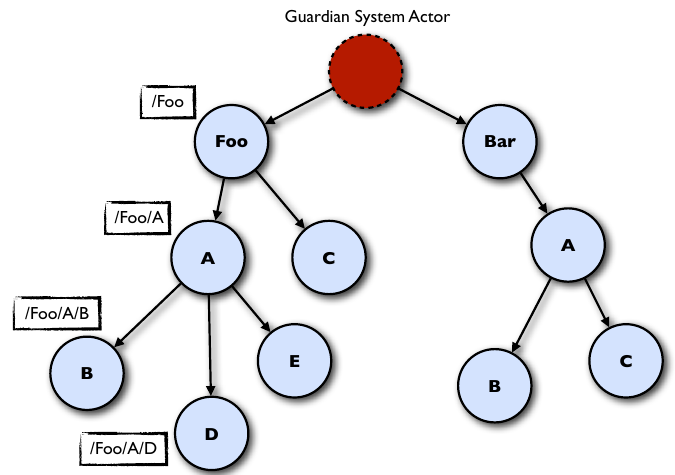
\includegraphics[scale=0.36]{./fig-actor-hierarchy.png}
  }
  \begin{center}
  \caption{A picture of the same gull
           looking the other way!}
  \end{center}
  
\end{figure}

\subsection{Rozproszenie.}
Aby rozproszyć system używając \mbox{Akka}, należy jedynie zmodyfikować jego konfigurację. Nie ruszamy zatem żadnej linii kodu. Konfiguracji podlega struktura hierarchii. Należy skonfigurować, jakie poddrzewo jest gdzie uruchamiane. Dla ilustacji $/Foo$ może dotyczyć jednej maszyny, a $/Bar$ drugiej. 

\subsection{Strategie nadzoru.}
Strategie nadzoru pozwalają na samoleczenie się systemu i poprawną obsługę błędów. Każdy rodzic ustala, jaka jest strategia nadzoru dla jego dzieci. Może to być Jeden-Za-Jeden lub Wszyscy-Za-Jednego. W przypadku Jeden-Za-Jeden, gdy aktor umrze, np. wskutek nieobsłużonego wyjątku, tylko ten aktor zostanie uruchomiony ponowie w nowym wcieleniu - a zatem ze stanem początkowym. W drugim przypadku wszystkie dzieci danego aktora zostaną uruchomione ponownie. Sama akcja, jak ponowne uruchomienie, to tylko przykład. Można wykonać dowolny kod, ale ponowne uruchomienie jest wbudowane w bibliotekę i często używane.

\section{Podsumowanie.}
Model aktorów jest prosty i zrozumiały. Pozwala na bezpiecznie programowanie współbieżne. Udostępnia nowy poziom abstrakcji - aktora. Pozwala tworzyć systemy, które w łatwy sposób mogą obsługiwać błędy aplikacji, sieciowe, sprzętowe. \mbox{Akka} ma wysoką wydajność, jest w pełni asynchroniczna i pozbawiona blokad. Pozwala na bardzo proste rozproszenie aplikacji. Istnieje do niej wiele rozszerzeń, np. do budowy klastra, do zapisu stanu aktora w bazie danych.

Moja praca magisterka dotyczy opracowania transakcji lub mechanizmu dającego podobny efekt dla rozproszonej bazy danych Apache Cassandra. Model aktorów pozwoli na stworzenie asynchronicznego, wysoko wydajnego rozproszonego sterownika transakcji.



%------------------------------------------------
%
%
%
%\section{Results}
%
%\begin{table}[H]
%\caption{Example table}
%\centering
%\begin{tabular}{llr}
%\toprule
%\multicolumn{2}{c}{Name} \\
%\cmidrule(r){1-2}
%First name & Last Name & Grade \\
%\midrule
%John & Doe & $7.5$ \\
%Richard & Miles & $2$ \\
%\bottomrule
%\end{tabular}
%\end{table}
%
%\lipsum[5] % Dummy text
%
%\begin{equation}
%\label{eq:emc}
%e = mc^2
%\end{equation}
%
%\lipsum[6] % Dummy text

%------------------------------------------------



%----------------------------------------------------------------------------------------
% REFERENCE LIST
%----------------------------------------------------------------------------------------

\bibliography{bibliography}{}
\bibliographystyle{plain}


%----------------------------------------------------------------------------------------

\end{multicols}

\end{document}